\documentclass[11pt,a4paper]{article}

\usepackage[utf8]{inputenc}
\usepackage[T1]{fontenc}
\usepackage[italian]{babel}
\usepackage{lmodern}
\usepackage{microtype}
\usepackage[a4paper,top=1.65cm,bottom=1.65cm,left=1.8cm,right=1.8cm]{geometry}
\usepackage{graphicx}
\usepackage{float}
\usepackage{caption}
\usepackage{tabularx}
\usepackage{booktabs}
\usepackage{array}
\usepackage{xcolor}
\usepackage{enumitem}
\usepackage{titlesec}
\usepackage{fancyhdr}
\usepackage{hyperref}

\definecolor{primary}{HTML}{1D4ED8}
\definecolor{dark}{HTML}{172554}
\definecolor{light}{HTML}{EFF6FF}
\definecolor{linegray}{HTML}{CBD5E1}

\hypersetup{colorlinks=true,linkcolor=dark,urlcolor=primary}
\setlength{\parindent}{0pt}
\setlength{\parskip}{4.2pt}
\setlength{\emergencystretch}{2em}
\raggedbottom

\titleformat{\section}{\Large\bfseries\color{dark}}{\thesection.}{0.55em}{}
\titlespacing*{\section}{0pt}{8pt}{4pt}
\titleformat{\subsection}{\normalsize\bfseries\color{dark}}{}{0pt}{}
\titlespacing*{\subsection}{0pt}{5pt}{2pt}

\captionsetup{font=small,labelfont=bf,skip=3pt}
\pagestyle{fancy}
\fancyhf{}
\lhead{Parking Spot}
\rhead{Raffaele Pio Sicilia}
\cfoot{\thepage}
\renewcommand{\headrulewidth}{0.4pt}
\setlength{\headheight}{14pt}

\newcolumntype{Y}{>{\raggedright\arraybackslash}X}
\newcommand{\patternrow}[2]{\textbf{#1} & #2 \\
}

\begin{document}

{\centering
{\LARGE\bfseries\color{dark} Analisi e descrizione dell'applicazione ``Parking Spot''\par}
\vspace{2pt}
}
\vspace{5pt}
\hrule
\vspace{4pt}

\section{Introduzione e contesto dell'applicazione}

Parking Spot è un'applicazione web per la gestione e la prenotazione di posti auto. Il sistema rappresenta un parcheggio composto da 87 posti, suddivisi nelle zone A e B, e permette di visualizzarne la disponibilità in una determinata fascia oraria attraverso una mappa 2D. L'utente deve registrarsi, successivamente può autenticarsi, completare il proprio profilo, associare uno o più veicoli e prenotare i posti disponibili nella fascia oraria che preferisce.

L'applicazione distingue, a livello di back-end, le funzionalità dell'utente da quelle amministrative. L'utente può consultare, creare e cancellare esclusivamente le proprie prenotazioni. L'amministratore, tramite endpoint REST protetti, può gestire i posti auto, consultare tutti gli utenti e visualizzare l'insieme delle prenotazioni. Nell'attuale front-end non è però presente una sezione amministrativa dedicata: tali operazioni sono quindi disponibili nelle API, ma non sono esposte dall'interfaccia grafica. L'autenticazione è delegata a Keycloak, mentre il back-end verifica il token JWT e applica i controlli di autorizzazione previsti per i ruoli \texttt{USER} e \texttt{ADMIN}.

\begin{figure}[H]
    \centering
    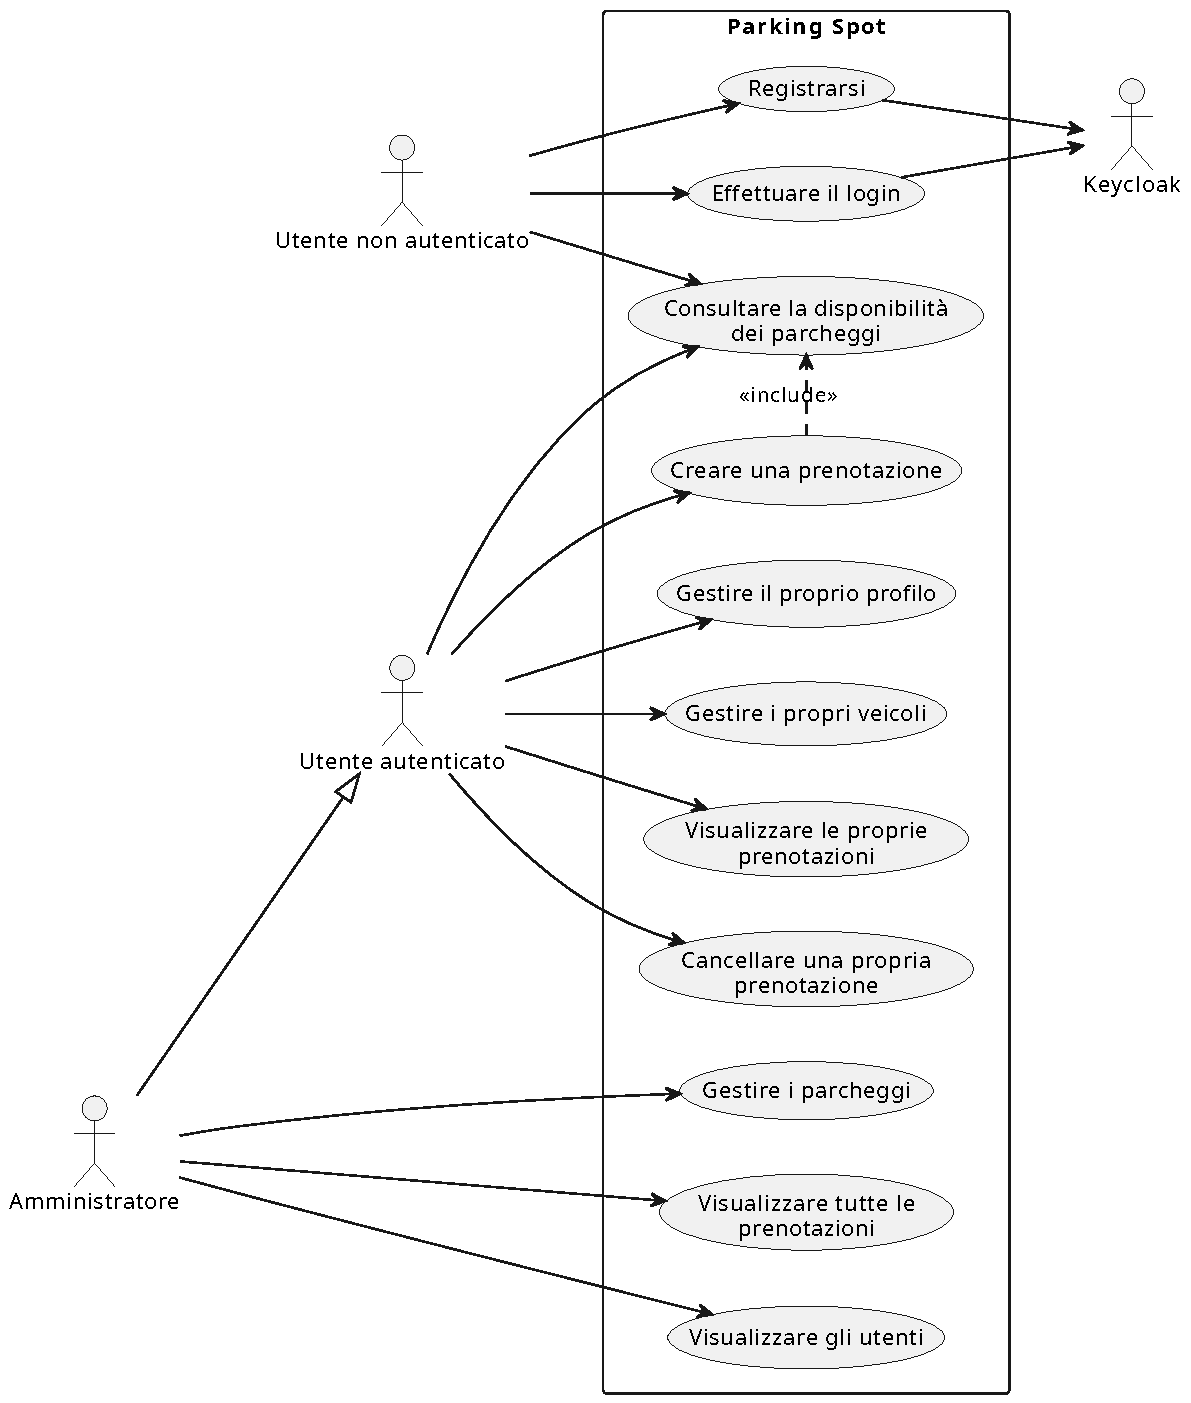
\includegraphics[width=0.59\textwidth]{diagrammi/pdf_progetto/use_case_diagram.pdf}
    \caption{Diagramma UML dei casi d'uso dell'applicazione.}
\end{figure}

\section{Analisi dei requisiti}

I requisiti funzionali principali comprendono la registrazione e il login, la gestione del profilo utente, l'inserimento dei veicoli, la ricerca dei posti disponibili per data e fascia oraria, la creazione di una prenotazione e la sua cancellazione. Il profilo è collegato all'identificativo Keycloak, l'email, il codice fiscale e la targa sono soggetti a vincoli di unicità. Le prenotazioni possono avere una durata compresa tra una e dodici ore e non possono riferirsi a una fascia oraria già trascorsa.

Tra i requisiti non funzionali rientrano la sicurezza, la consistenza dei dati e la gestione della concorrenza. Il back-end è stateless e accetta Token Bearer firmati dal realm Keycloak, le API amministrative sono protette mediante il controllo del ruolo. Le operazioni di prenotazione verificano la sovrapposizione temporale sia sul posto auto, sia sul veicolo. Il lock pessimistico acquisito sui record del parcheggio e del veicolo, insieme ai controlli di sovrapposizione eseguiti nella stessa transazione, impedisce che due richieste concorrenti prenotino lo stesso posto o impieghino lo stesso veicolo nella medesima fascia oraria. L'entità \texttt{Parcheggio} contiene anche un campo \texttt{@Version}, utilizzato da JPA per il controllo ottimistico quando il record viene effettivamente aggiornato, la creazione di una prenotazione, tuttavia, non modifica tale record e si basa principalmente sui lock pessimistici e sulle query di sovrapposizione.

\section{Back-end e tecnologie impiegate}

Il back-end è sviluppato in Java 17 con Spring Boot e utilizza Spring Web MVC per le API REST, Spring Data JPA per la persistenza, Spring Validation per il controllo dei dati e Spring Security OAuth2 Resource Server per la validazione dei JWT. Il database PostgreSQL conserva utenti, veicoli, parcheggi e prenotazioni. PostgreSQL e Keycloak vengono avviati mediante Docker Compose, mentre Hibernate aggiorna lo schema a partire dalle entità JPA.

L'applicazione adotta un'architettura a livelli. 

I Controller ricevono le richieste HTTP e delegano l'elaborazione ai servizi. 

I Service contengono la logica applicativa e delimitano le transazioni. 

I Repository incapsulano l'accesso ai dati. 

Le Entity principali sono \texttt{Utente}, \texttt{Veicolo}, \texttt{Parcheggio} e \texttt{Prenotazione}. Ogni prenotazione collega un utente, un veicolo e un posto auto.

Sono inoltre utilizzati DTO di richiesta e risposta, che separano il modello persistente dai dati scambiati con il client.

\subsection{Metodi HTTP esposti dalle API REST}

Le API utilizzano i principali metodi del protocollo HTTP secondo le operazioni richieste sulle risorse del sistema.

\begin{table}[H]
\centering
\scriptsize
\begin{tabularx}{\textwidth}{
>{\raggedright\arraybackslash\bfseries}p{1.45cm}
>{\raggedright\arraybackslash}p{7.95cm}
Y}
\toprule
Metodo & Endpoint & Funzione principale \\
\midrule
GET &
\texttt{/api/auth/me};
\texttt{/api/parcheggi};
\texttt{/api/parcheggi/disponibili};
\texttt{/api/parcheggi/disponibilita};
\texttt{/api/parcheggi/\{id\}};
\texttt{/api/prenotazioni};
\texttt{/api/prenotazioni/admin};
\texttt{/api/utenti/me};
\texttt{/api/utenti};
\texttt{/api/utenti/\{id\}};
\texttt{/api/veicoli}
&
Consultazione dell'utente autenticato, dei parcheggi, della disponibilità, delle prenotazioni, dei profili e dei veicoli. Gli endpoint amministrativi richiedono il ruolo \texttt{ADMIN}. \\

POST &
\texttt{/api/parcheggi};
\texttt{/api/prenotazioni};
\texttt{/api/utenti/me};
\texttt{/api/veicoli}
&
Creazione di un parcheggio, di una prenotazione, del profilo personale e di un veicolo. La creazione dei parcheggi è riservata all'amministratore. \\

PUT &
\texttt{/api/parcheggi/\{id\}}
&
Aggiornamento completo dei dati di un parcheggio, consentito esclusivamente all'amministratore. \\

DELETE &
\texttt{/api/parcheggi/\{id\}};
\texttt{/api/prenotazioni/\{id\}};
\texttt{/api/veicoli/\{id\}}
&
Eliminazione di un parcheggio oppure cancellazione di una prenotazione o di un veicolo appartenenti all'utente autenticato. \\
\bottomrule
\end{tabularx}
\caption{Principali metodi HTTP ed endpoint REST esposti dal back-end.}
\end{table}

Sono inoltre presenti due endpoint \texttt{PATCH}, riservati all'amministratore:
\begin{center}
\footnotesize
\texttt{PATCH /api/parcheggi/\{numero\}/abilita}\\
\texttt{PATCH /api/parcheggi/\{numero\}/disabilita}
\end{center}
Tali endpoint consentono di modificare lo stato operativo di un posto auto.


\subsection{Pattern architetturali e applicativi nel back-end}

Nel back-end sono riconoscibili alcuni pattern architetturali e applicativi utilizzati per separare le responsabilità e ridurre l'accoppiamento tra i componenti. Non si tratta esclusivamente di design pattern GoF, ma di pattern tipici delle applicazioni enterprise.

\begin{table}[H]
\centering
\footnotesize
\begin{tabularx}{\textwidth}{>{\raggedright\arraybackslash\bfseries}p{3.65cm}Y}
\toprule
Pattern & Applicazione nel progetto \\
\midrule
Layered Architecture & Il sistema è suddiviso nei livelli Controller, Service, Repository ed Entity. Ogni livello svolge una responsabilità specifica e comunica con quello immediatamente successivo. \\
Repository & Le interfacce che estendono \texttt{JpaRepository} costituiscono il punto di accesso ai dati e nascondono ai servizi i dettagli delle operazioni di persistenza e delle query. \\
Service Layer & Le classi di servizio concentrano la logica applicativa, le validazioni, i controlli di autorizzazione e il coordinamento delle operazioni transazionali. \\
Data Transfer Object & I DTO di richiesta e risposta trasferiscono i dati tra client e back-end senza esporre direttamente le entità JPA, riducendo l'accoppiamento tra API REST e modello persistente. \\
\bottomrule
\end{tabularx}
\end{table}

Le dipendenze tra Controller, Service e Repository sono gestite da Spring mediante la \textbf{Dependency Injection} tramite costruttore. In questo modo, ogni componente riceve dall’esterno le risorse necessarie al proprio funzionamento, senza doverle creare direttamente. Tale meccanismo riduce l’accoppiamento tra le classi e migliora la modularità, la manutenibilità e la testabilità del codice.

La creazione della prenotazione è l'operazione transazionale più delicata. Il Service valida la fascia oraria, identifica l'utente dal JWT, acquisisce un lock pessimistico sul posto auto e sul veicolo e controlla eventuali sovrapposizioni. Solo al termine dei controlli viene salvata l'entità e viene effettuato il commit della transazione. In presenza di errori, l'operazione viene annullata e il client riceve uno stato HTTP coerente.

\begin{figure}[H]
    \centering
    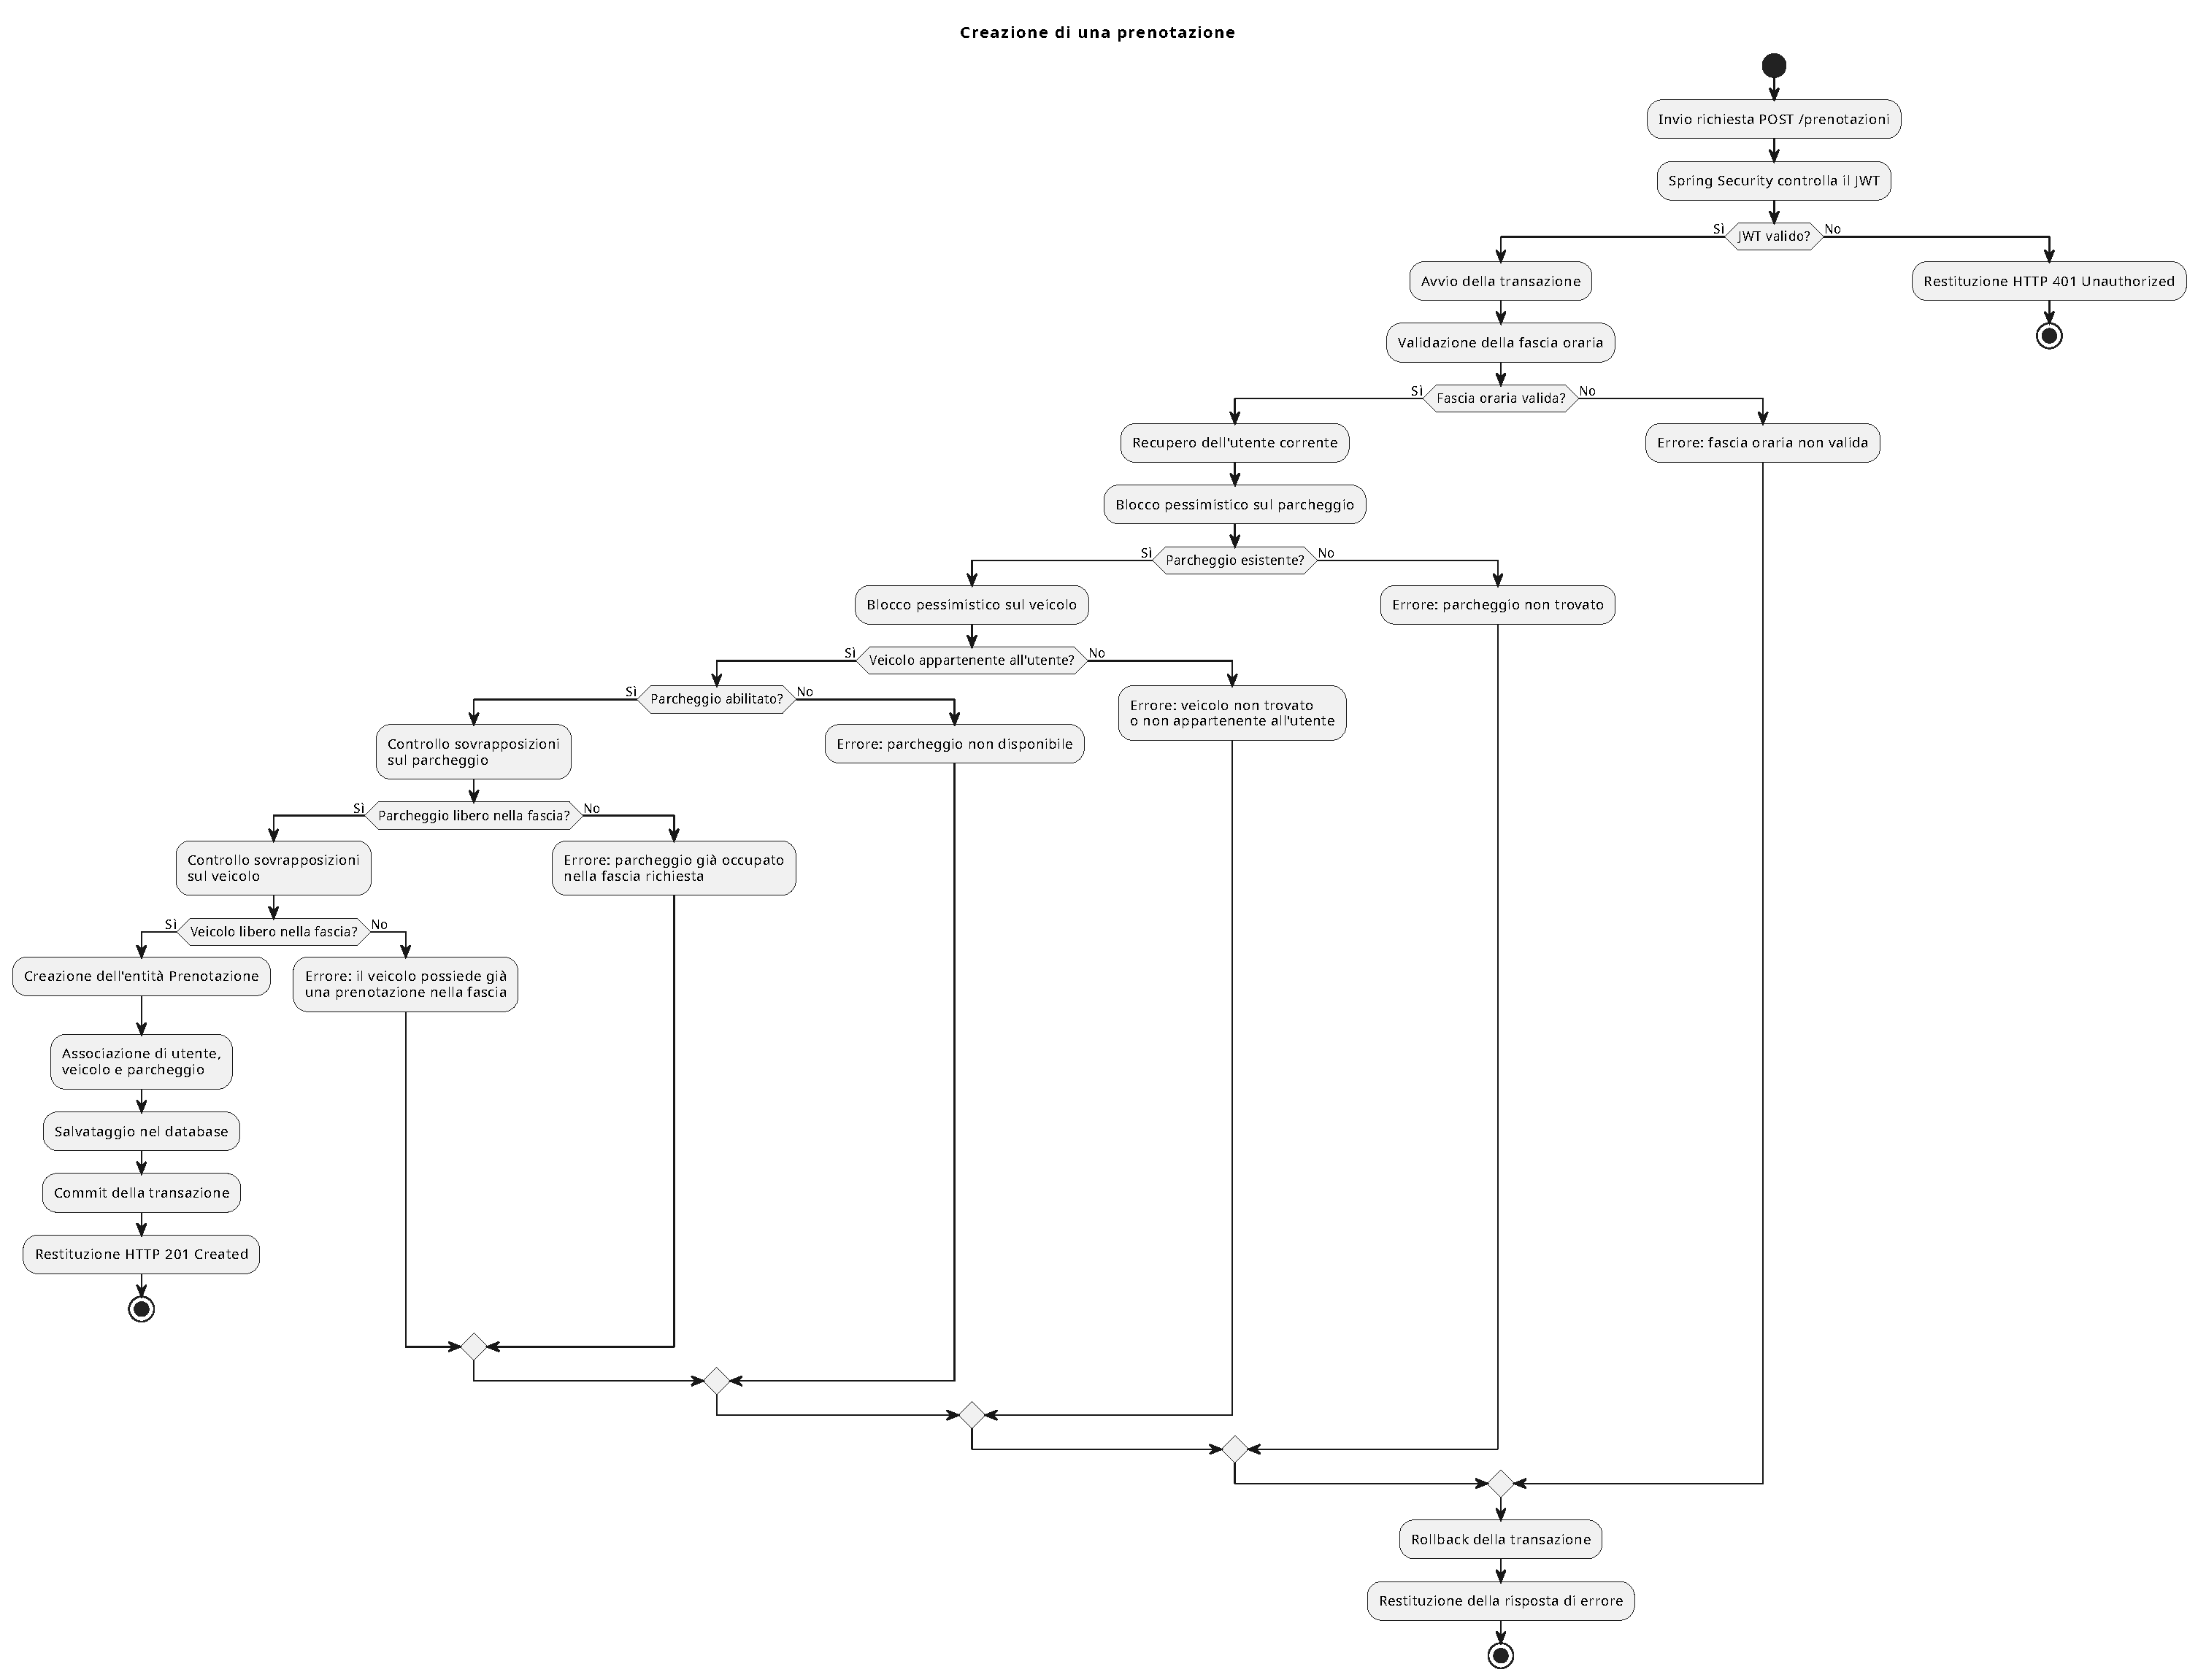
\includegraphics[width=0.62\textwidth]{diagrammi/pdf_progetto/flow_creazione_prenotazione.pdf}
    \caption{Activity Diagram UML della creazione di una prenotazione.}
\end{figure}

La cancellazione della prenotazione è anch'essa racchiusa in una transazione. La ricerca avviene tramite identificativo della prenotazione e proprietario corrente, in modo che un utente non possa eliminare prenotazioni appartenenti ad altri. Se la risorsa non viene trovata viene restituito un errore HTTP 404, in caso contrario il repository esegue l'eliminazione e la transazione termina con una risposta 204.

\begin{figure}[H]
    \centering
    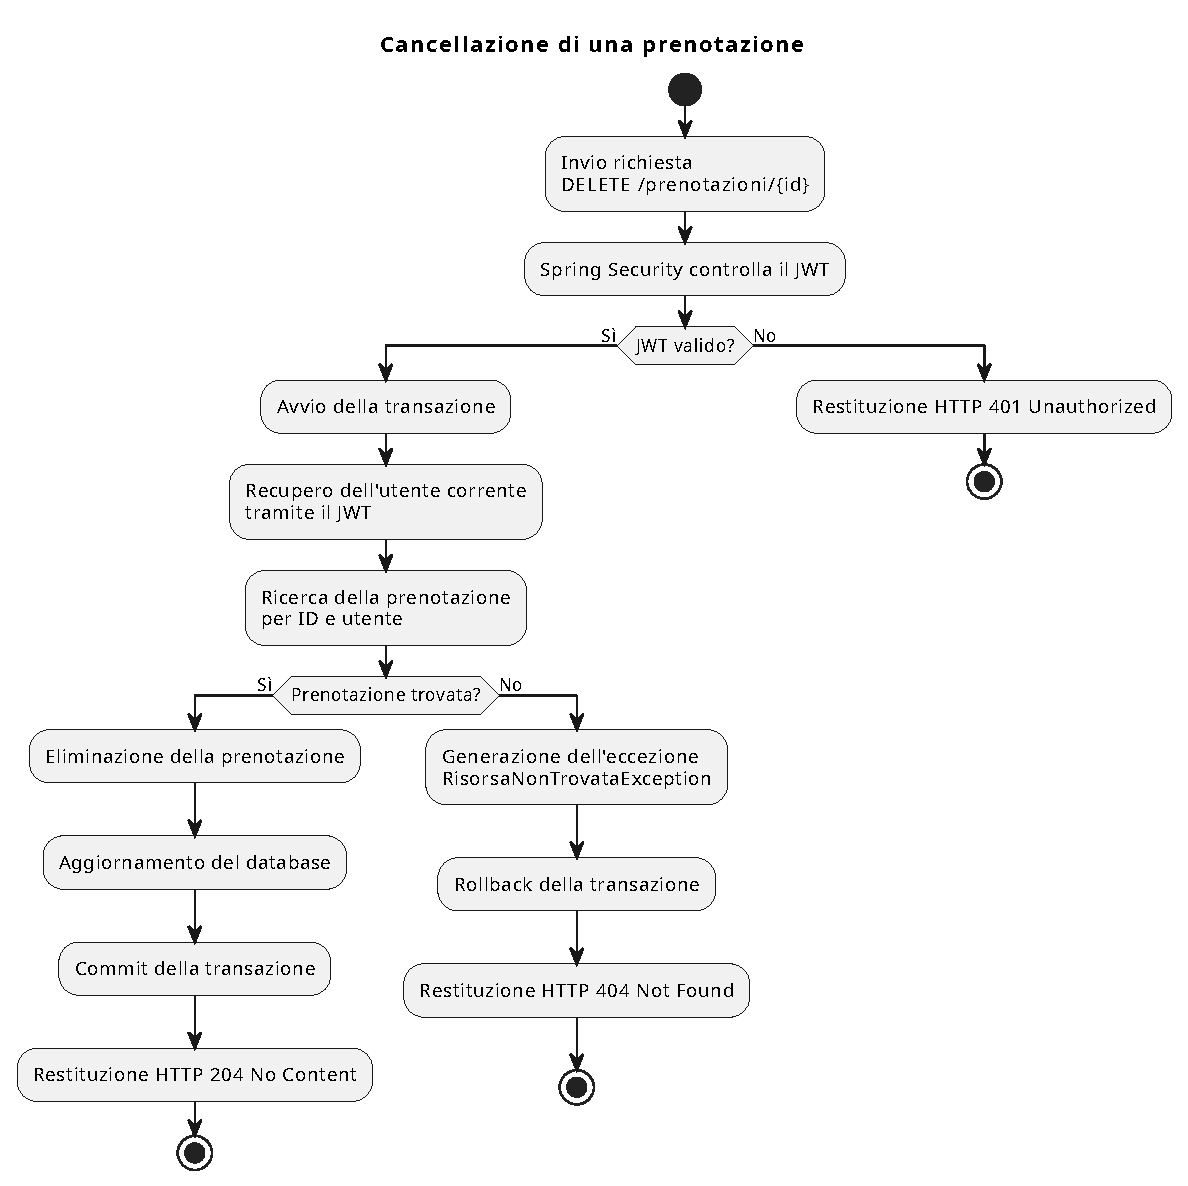
\includegraphics[width=0.38\textwidth]{diagrammi/pdf_progetto/flow_cancellazione_prenotazione.pdf}
    \caption{Activity Diagram UML della cancellazione di una prenotazione.}
\end{figure}

La gestione degli errori è centralizzata tramite \texttt{@RestControllerAdvice}, che traduce eccezioni applicative, conflitti di integrità e problemi di concorrenza in risposte HTTP strutturate. La consistenza è inoltre garantita dai vincoli di unicità, dalle associazioni obbligatorie tra le entità e dalle query che rilevano le sovrapposizioni temporali. 
All'avvio è presente un inizializzatore che completa i posti fino al numero 87 evitando duplicati.

\section{Front-end e tecnologie impiegate}

Il front-end è realizzato con Angular mediante un componente standalone. L'interfaccia utilizza FormsModule per il binding dei moduli, HttpClient per le richieste REST e RxJS per la gestione asincrona delle risposte. La libreria \texttt{keycloak-js} avvia la sessione Single Sign-On, esegue login, registrazione e logout e rende disponibile il token da allegare alle richieste protette.

La pagina iniziale presenta l'accesso e la registrazione. Dopo aver effettuato il login, viene mostrata una dashboard composta da due sezioni: ``Prenotazioni e mappa'' e ``Profilo e veicoli''. Nella prima l'utente sceglie data, ora, durata e veicolo e la risposta del back-end viene rappresentata sulla planimetria con colori diversi per posti liberi, occupati e per le categorie grafiche ``disabili'' e ``scarico merci''. Nella seconda sezione vengono gestiti i dati anagrafici e i veicoli associati al profilo.

\subsection{Pattern progettuali nel front-end}

Nel front-end i pattern sono applicati soprattutto nei servizi Angular e nella gestione asincrona delle comunicazioni con il back-end.

\begin{table}[H]
\centering
\footnotesize
\begin{tabularx}{\textwidth}{>{\raggedright\arraybackslash\bfseries}p{3.35cm}Y}
\toprule
Pattern & Applicazione nel progetto \\
\midrule
Singleton & \texttt{KeycloakService} e \texttt{ParkingApiService} sono dichiarati con \texttt{providedIn: 'root'}. L'injector principale di Angular mantiene quindi una sola istanza condivisa di ciascun servizio per tutta l'applicazione. \\
Facade & \texttt{ParkingApiService} svolge un ruolo assimilabile a una Facade, poiché espone al componente un punto di accesso unitario alle operazioni su profilo, veicoli, parcheggi e prenotazioni, nascondendo URL, parametri e dettagli delle chiamate HTTP. Anche \texttt{KeycloakService} incapsula l'interazione con la libreria \texttt{keycloak-js}. \\
Interceptor & L'\texttt{authInterceptor} intercetta le richieste HTTP dirette al back-end e aggiunge automaticamente l'header \texttt{Authorization} con il Token Bearer, evitando di ripetere questa operazione in ogni chiamata. \\
Observer & Le operazioni di \texttt{HttpClient} restituiscono \texttt{Observable}. Il componente si sottoscrive con \texttt{subscribe()} e reagisce alla ricezione dei dati o alla presenza di errori, secondo il meccanismo del pattern Observer. \\
\bottomrule
\end{tabularx}
\end{table}

\begin{figure}[H]
    \centering
    \begin{minipage}[t]{0.49\textwidth}
        \centering
        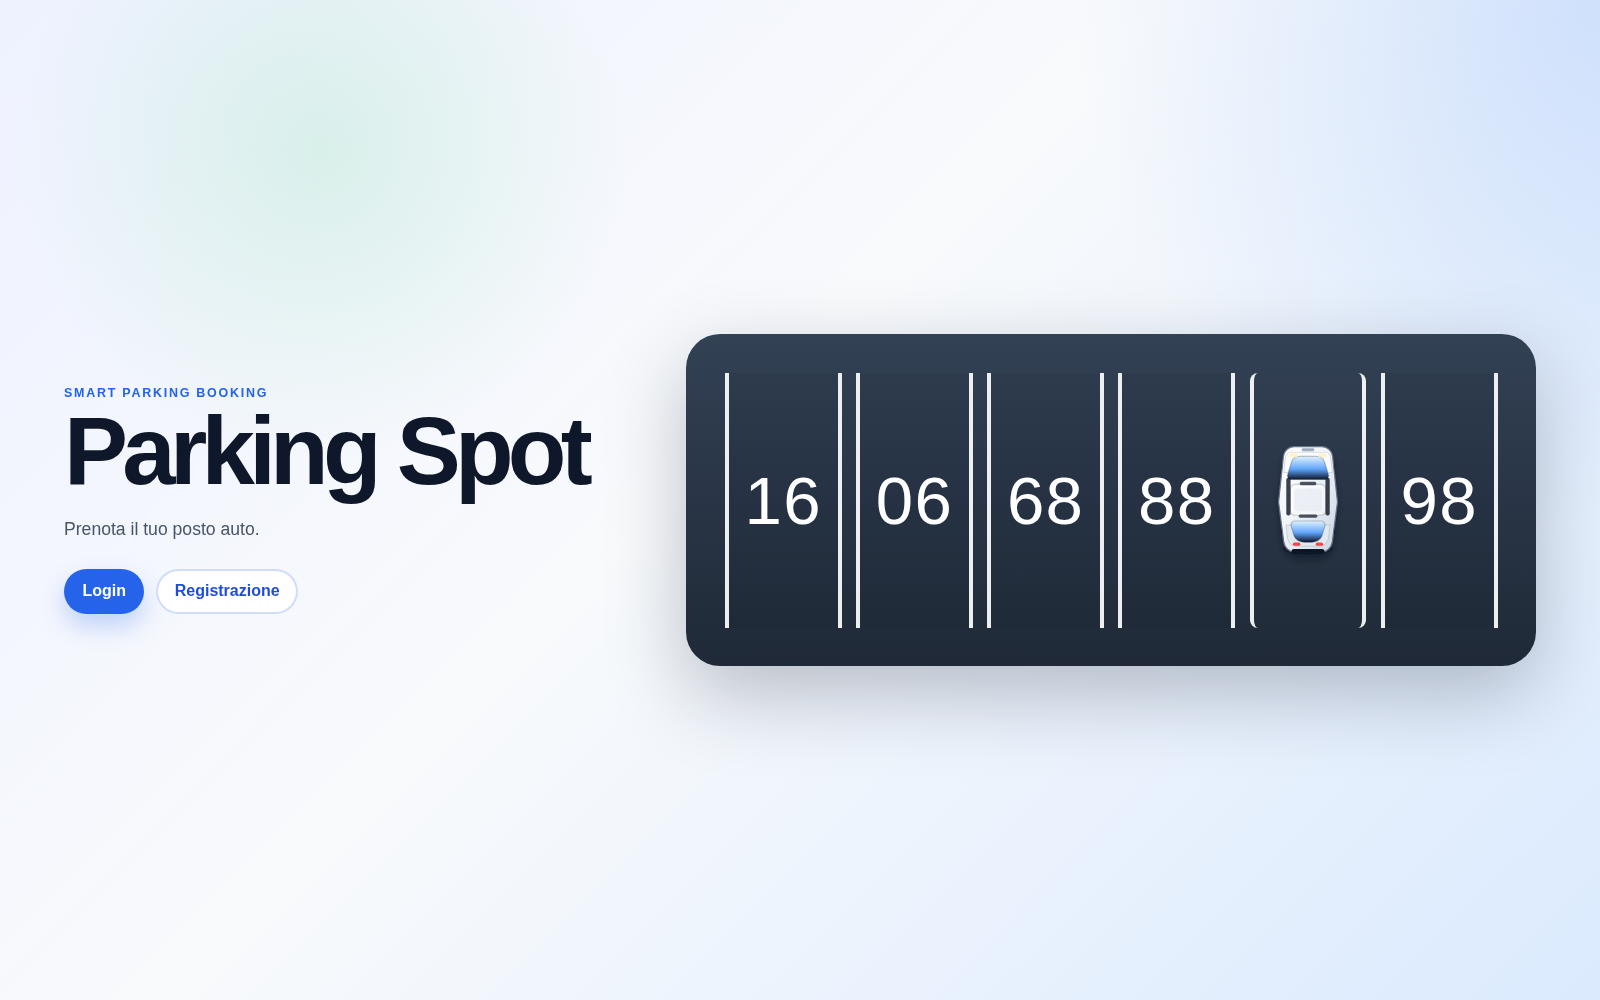
\includegraphics[width=\linewidth]{immagini/01_accesso.png}
        \caption*{(a) Pagina di accesso e registrazione.}
    \end{minipage}\hfill
    \begin{minipage}[t]{0.49\textwidth}
        \centering
        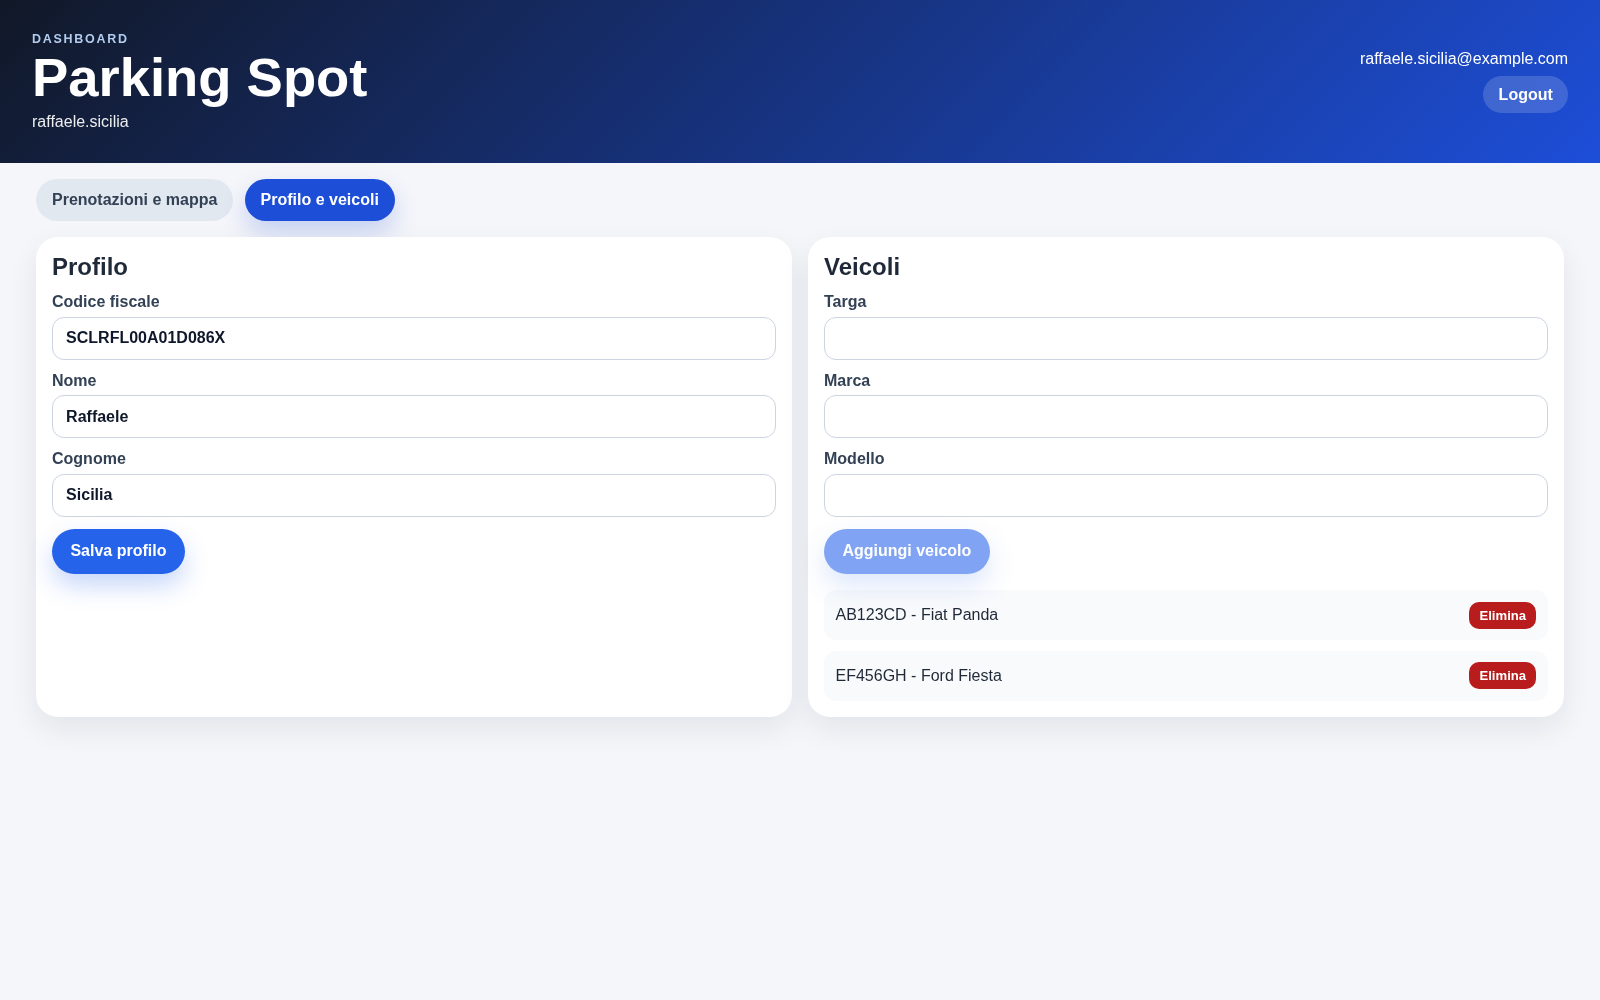
\includegraphics[width=\linewidth]{immagini/03_profilo.png}
        \caption*{(b) Gestione del profilo e dei veicoli.}
    \end{minipage}
    \caption{Principali schermate di autenticazione e gestione dei dati personali.}
\end{figure}

La mappa 2D è costruita a partire dai dati restituiti dall'endpoint di disponibilità. I posti vengono ordinati per numero e arricchiti sul client con zona, tipologia e posizione grafica. Le tipologie ``disabili'' e ``scarico merci'' sono quindi informazioni definite esclusivamente nel front-end in base al numero del posto, non sono memorizzate nel database e non vengono validate dal back-end. Di conseguenza, i posti rappresentati come riservati ai disabili restano prenotabili come posti ordinari, mentre quelli mostrati come area di scarico merci vengono resi non prenotabili soltanto dall'interfaccia grafica. I pulsanti ``Zona A'' e ``Zona B'' permettono di concentrare la visualizzazione su una singola area, mentre la legenda rende immediata l'interpretazione dello stato di ogni posto. Il pulsante di prenotazione viene disabilitato quando il posto non è prenotabile, non è disponibile oppure mancano profilo o veicolo.

\begin{figure}[H]
    \centering
    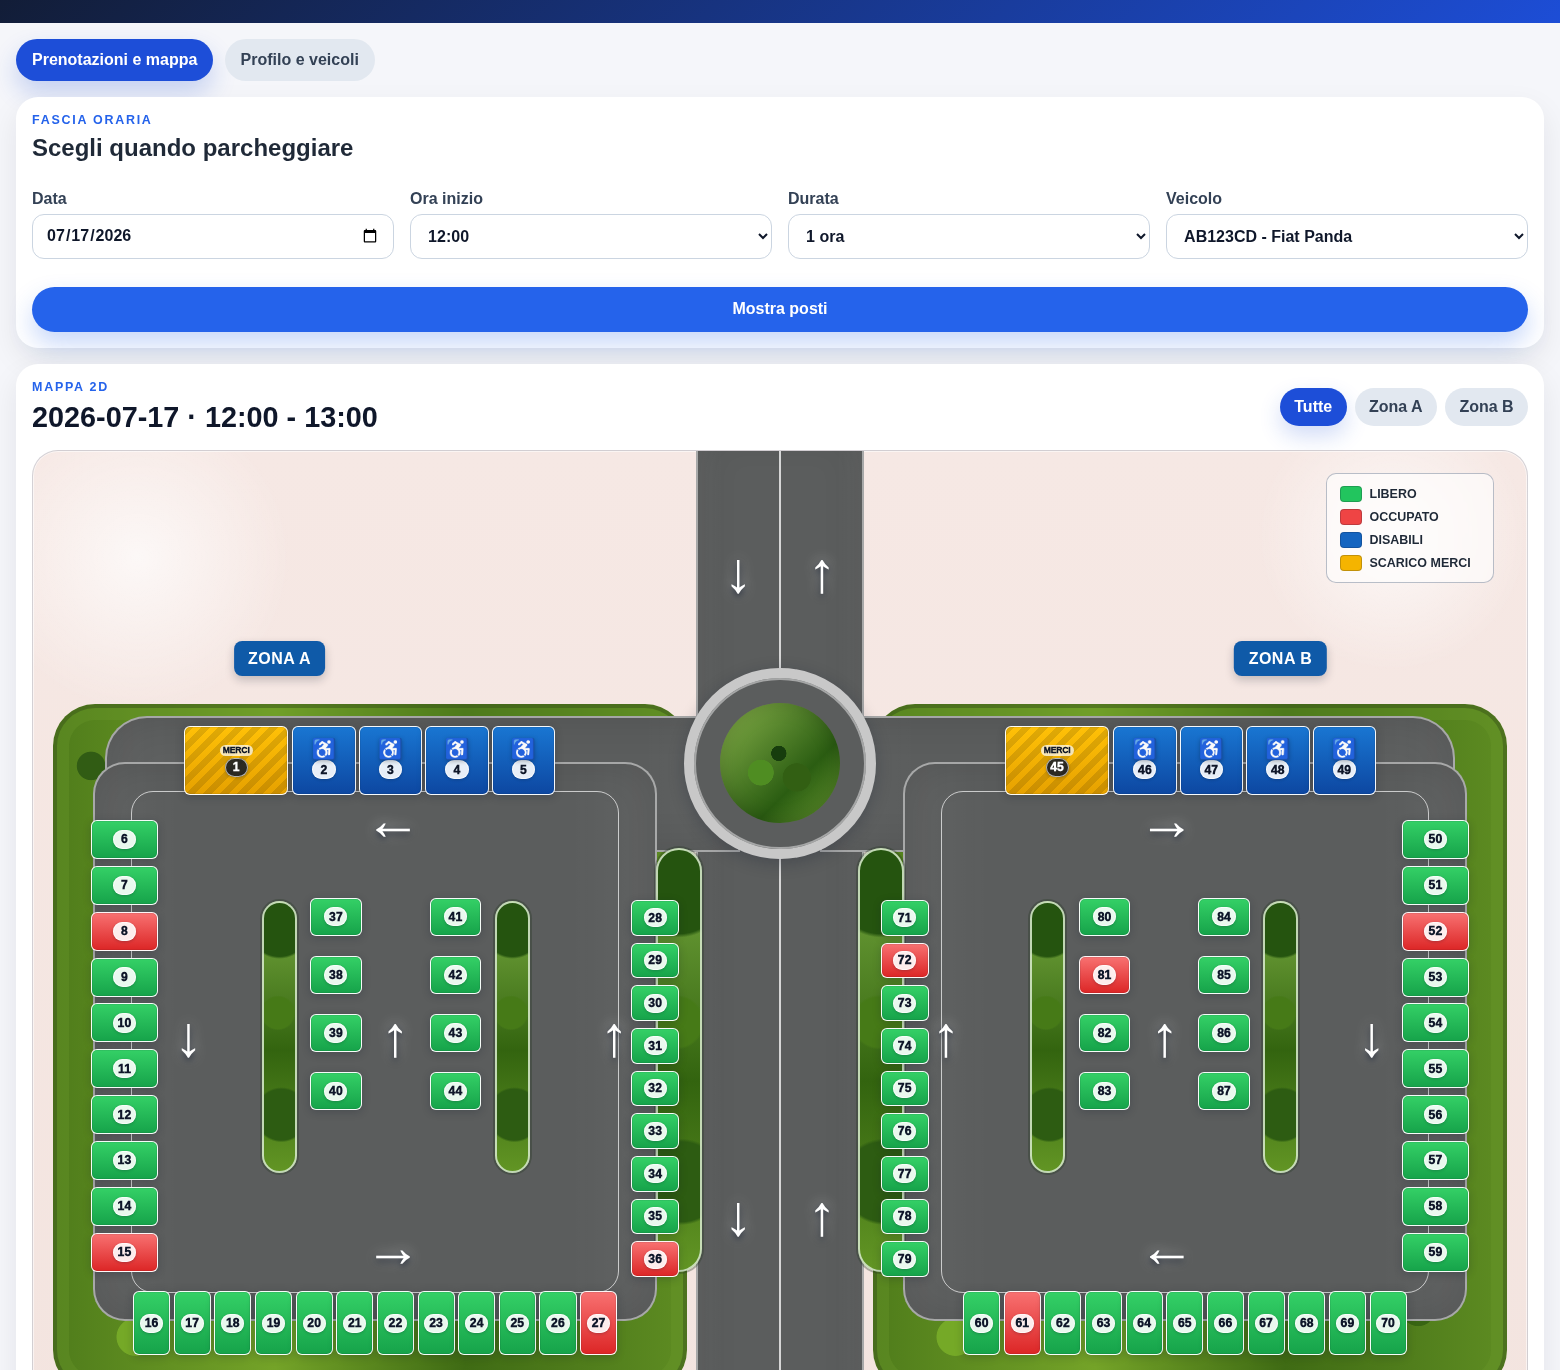
\includegraphics[width=0.94\textwidth]{immagini/02_mappa.png}
    \caption{Ricerca della disponibilità e mappa bidimensionale del parcheggio.}
\end{figure}

\section{Conclusioni}

Parking Spot realizza un flusso completo di autenticazione, gestione dei dati personali e prenotazione temporale dei posti auto. La separazione tra Angular, API REST, Service, Repository, PostgreSQL e Keycloak rende il progetto modulare e facilita la manutenzione. I controlli di unicità, autorizzazione, sovrapposizione e concorrenza garantiscono una gestione coerente delle prenotazioni anche in presenza di richieste simultanee.

Gli sviluppi successivi potrebbero riguardare l'uso di HTTPS, una sezione ampia di test automatici, notifiche sulle prenotazioni, strumenti amministrativi dedicati nel front-end.

\end{document}
